%%%%%%%%%%%%%%%%%%%%%%%%%%%%%%%%%%%%%%%%%
%  My documentation report
%  Objetive: Explain what I did and how, so someone can continue with the investigation
%
% Important note:
% Chapter heading images should have a 2:1 width:height ratio,
% e.g. 920px width and 460px height.
%
%%%%%%%%%%%%%%%%%%%%%%%%%%%%%%%%%%%%%%%%%

%----------------------------------------------------------------------------------------
%	PACKAGES AND OTHER DOCUMENT CONFIGURATIONS
%----------------------------------------------------------------------------------------

\documentclass[11pt,fleqn]{book} % Default font size and left-justified equations

\usepackage[top=3cm,bottom=3cm,left=3.2cm,right=3.2cm,headsep=10pt,letterpaper]{geometry} % Page margins

\usepackage{xcolor} % Required for specifying colors by name
\definecolor{darkgreen}{RGB}{0, 153, 0} % Define the orange color used for highlighting throughout the book

% Font Settings
\usepackage{avant} % Use the Avantgarde font for headings
%\usepackage{times} % Use the Times font for headings
\usepackage{mathptmx} % Use the Adobe Times Roman as the default text font together with math symbols from the Sym­bol, Chancery and Com­puter Modern fonts

\usepackage{microtype} % Slightly tweak font spacing for aesthetics
\usepackage[utf8]{inputenc} % Required for including letters with accents
\usepackage[T1]{fontenc} % Use 8-bit encoding that has 256 glyphs
\usepackage{float}

% Bibliography
\usepackage[style=alphabetic,sorting=nyt,sortcites=true,autopunct=true,babel=hyphen,hyperref=true,abbreviate=false,backref=true,backend=biber]{biblatex}
\addbibresource{bibliography.bib} % BibTeX bibliography file
\defbibheading{bibempty}{}

%----------------------------------------------------------------------------------------
%	VARIOUS REQUIRED PACKAGES
%----------------------------------------------------------------------------------------

\usepackage{titlesec} % Allows customization of titles

\usepackage{graphicx} % Required for including pictures
\graphicspath{{Pictures/}} % Specifies the directory where pictures are stored

\usepackage{lipsum} % Inserts dummy text

\usepackage{tikz} % Required for drawing custom shapes

\usepackage[english]{babel} % English language/hyphenation

\usepackage{enumitem} % Customize lists
\setlist{nolistsep} % Reduce spacing between bullet points and numbered lists

\usepackage{booktabs} % Required for nicer horizontal rules in tables

\usepackage{eso-pic} % Required for specifying an image background in the title page

%----------------------------------------------------------------------------------------
%	MAIN TABLE OF CONTENTS
%----------------------------------------------------------------------------------------

\usepackage{titletoc} % Required for manipulating the table of contents

\contentsmargin{0cm} % Removes the default margin
% Chapter text styling
\titlecontents{chapter}[1.25cm] % Indentation
{\addvspace{15pt}\large\sffamily\bfseries} % Spacing and font options for chapters
{\color{darkgreen!60}\contentslabel[\Large\thecontentslabel]{1.25cm}\color{darkgreen}} % Chapter number
{}  
{\color{darkgreen!60}\normalsize\sffamily\bfseries\;\titlerule*[.5pc]{.}\;\thecontentspage} % Page number
% Section text styling
\titlecontents{section}[1.25cm] % Indentation
{\addvspace{5pt}\sffamily\bfseries} % Spacing and font options for sections
{\contentslabel[\thecontentslabel]{1.25cm}} % Section number
{}
{\sffamily\hfill\color{black}\thecontentspage} % Page number
[]
% Subsection text styling
\titlecontents{subsection}[1.25cm] % Indentation
{\addvspace{1pt}\sffamily\small} % Spacing and font options for subsections
{\contentslabel[\thecontentslabel]{1.25cm}} % Subsection number
{}
{\sffamily\;\titlerule*[.5pc]{.}\;\thecontentspage} % Page number
[] 

%----------------------------------------------------------------------------------------
%	MINI TABLE OF CONTENTS IN CHAPTER HEADS
%----------------------------------------------------------------------------------------

% Section text styling
\titlecontents{lsection}[0em] % Indendating
{\footnotesize\sffamily} % Font settings
{}
{}
{}

% Subsection text styling
\titlecontents{lsubsection}[.5em] % Indentation
{\normalfont\footnotesize\sffamily} % Font settings
{}
{}
{}
 
%----------------------------------------------------------------------------------------
%	PAGE HEADERS
%----------------------------------------------------------------------------------------

\usepackage{fancyhdr} % Required for header and footer configuration

\pagestyle{fancy}
\renewcommand{\chaptermark}[1]{\markboth{\sffamily\normalsize\bfseries\chaptername\ \thechapter.\ #1}{}} % Chapter text font settings
\renewcommand{\sectionmark}[1]{\markright{\sffamily\normalsize\thesection\hspace{5pt}#1}{}} % Section text font settings
\fancyhf{} \fancyhead[LE,RO]{\sffamily\normalsize\thepage} % Font setting for the page number in the header
\fancyhead[LO]{\rightmark} % Print the nearest section name on the left side of odd pages
\fancyhead[RE]{\leftmark} % Print the current chapter name on the right side of even pages
\renewcommand{\headrulewidth}{0.5pt} % Width of the rule under the header
\addtolength{\headheight}{2.5pt} % Increase the spacing around the header slightly
\renewcommand{\footrulewidth}{0pt} % Removes the rule in the footer
\fancypagestyle{plain}{\fancyhead{}\renewcommand{\headrulewidth}{0pt}} % Style for when a plain pagestyle is specified

% Removes the header from odd empty pages at the end of chapters
\makeatletter
\renewcommand{\cleardoublepage}{
\clearpage\ifodd\c@page\else
\hbox{}
\vspace*{\fill}
\thispagestyle{empty}
\newpage
\fi}

%----------------------------------------------------------------------------------------
%	THEOREM STYLES
%----------------------------------------------------------------------------------------

\usepackage{amsmath,amsfonts,amssymb,amsthm} % For math equations, theorems, symbols, etc

\newcommand{\intoo}[2]{\mathopen{]}#1\,;#2\mathclose{[}}
\newcommand{\ud}{\mathop{\mathrm{{}d}}\mathopen{}}
\newcommand{\intff}[2]{\mathopen{[}#1\,;#2\mathclose{]}}
\newtheorem{notation}{Notation}[chapter]

%%%%%%%%%%%%%%%%%%%%%%%%%%%%%%%%%%%%%%%%%%%%%%%%%%%%%%%%%%%%%%%%%%%%%%%%%%%
%%%%%%%%%%%%%%%%%%%% dedicated to boxed/framed environements %%%%%%%%%%%%%%
%%%%%%%%%%%%%%%%%%%%%%%%%%%%%%%%%%%%%%%%%%%%%%%%%%%%%%%%%%%%%%%%%%%%%%%%%%%
\newtheoremstyle{ocrenumbox}% % Theorem style name
{0pt}% Space above
{0pt}% Space below
{\normalfont}% % Body font
{}% Indent amount
{\small\bf\sffamily\color{darkgreen}}% % Theorem head font
{\;}% Punctuation after theorem head
{0.25em}% Space after theorem head
{\small\sffamily\color{darkgreen}\thmname{#1}\nobreakspace\thmnumber{\@ifnotempty{#1}{}\@upn{#2}}% Theorem text (e.g. Theorem 2.1)
\thmnote{\nobreakspace\the\thm@notefont\sffamily\bfseries\color{black}---\nobreakspace#3.}} % Optional theorem note
\renewcommand{\qedsymbol}{$\blacksquare$}% Optional qed square

\newtheoremstyle{blacknumex}% Theorem style name
{5pt}% Space above
{5pt}% Space below
{\normalfont}% Body font
{} % Indent amount
{\small\bf\sffamily}% Theorem head font
{\;}% Punctuation after theorem head
{0.25em}% Space after theorem head
{\small\sffamily{\tiny\ensuremath{\blacksquare}}\nobreakspace\thmname{#1}\nobreakspace\thmnumber{\@ifnotempty{#1}{}\@upn{#2}}% Theorem text (e.g. Theorem 2.1)
\thmnote{\nobreakspace\the\thm@notefont\sffamily\bfseries---\nobreakspace#3.}}% Optional theorem note

\newtheoremstyle{blacknumbox} % Theorem style name
{0pt}% Space above
{0pt}% Space below
{\normalfont}% Body font
{}% Indent amount
{\small\bf\sffamily}% Theorem head font
{\;}% Punctuation after theorem head
{0.25em}% Space after theorem head
{\small\sffamily\thmname{#1}\nobreakspace\thmnumber{\@ifnotempty{#1}{}\@upn{#2}}% Theorem text (e.g. Theorem 2.1)
\thmnote{\nobreakspace\the\thm@notefont\sffamily\bfseries---\nobreakspace#3.}}% Optional theorem note

%%%%%%%%%%%%%%%%%%%%%%%%%%%%%%%%%%%%%%%%%%%%%%%%%%%%%%%%%%%%%%%%%%%%%%%%%%%
%%%%%%%%%%%%% dedicated to non-boxed/non-framed environements %%%%%%%%%%%%%
%%%%%%%%%%%%%%%%%%%%%%%%%%%%%%%%%%%%%%%%%%%%%%%%%%%%%%%%%%%%%%%%%%%%%%%%%%%
\newtheoremstyle{ocrenum}% % Theorem style name
{5pt}% Space above
{5pt}% Space below
{\normalfont}% % Body font
{}% Indent amount
{\small\bf\sffamily\color{darkgreen}}% % Theorem head font
{\;}% Punctuation after theorem head
{0.25em}% Space after theorem head
{\small\sffamily\color{darkgreen}\thmname{#1}\nobreakspace\thmnumber{\@ifnotempty{#1}{}\@upn{#2}}% Theorem text (e.g. Theorem 2.1)
\thmnote{\nobreakspace\the\thm@notefont\sffamily\bfseries\color{black}---\nobreakspace#3.}} % Optional theorem note
\renewcommand{\qedsymbol}{$\blacksquare$}% Optional qed square
\makeatother

% Defines the theorem text style for each type of theorem to one of the three styles above
\newcounter{dummy} 
\numberwithin{dummy}{section}
\theoremstyle{ocrenumbox}
\newtheorem{theoremeT}[dummy]{Theorem}
\newtheorem{problem}{Problem}[chapter]
\newtheorem{exerciseT}{Exercise}[chapter]
\theoremstyle{blacknumex}
\newtheorem{exampleT}{Example}[chapter]
\theoremstyle{blacknumbox}
\newtheorem{vocabulary}{Vocabulary}[chapter]
\newtheorem{definitionT}{Definition}[section]
\newtheorem{corollaryT}[dummy]{Corollary}
\theoremstyle{ocrenum}
\newtheorem{proposition}[dummy]{Proposition}

%----------------------------------------------------------------------------------------
%	DEFINITION OF COLORED BOXES
%----------------------------------------------------------------------------------------

\RequirePackage[framemethod=default]{mdframed} % Required for creating the theorem, definition, exercise and corollary boxes

% Theorem box
\newmdenv[skipabove=7pt,
skipbelow=7pt,
backgroundcolor=black!5,
linecolor=darkgreen,
innerleftmargin=5pt,
innerrightmargin=5pt,
innertopmargin=5pt,
leftmargin=0cm,
rightmargin=0cm,
innerbottommargin=5pt]{tBox}

% Exercise box	  
\newmdenv[skipabove=7pt,
skipbelow=7pt,
rightline=false,
leftline=true,
topline=false,
bottomline=false,
backgroundcolor=darkgreen!10,
linecolor=darkgreen,
innerleftmargin=5pt,
innerrightmargin=5pt,
innertopmargin=5pt,
innerbottommargin=5pt,
leftmargin=0cm,
rightmargin=0cm,
linewidth=4pt]{eBox}	

% Definition box
\newmdenv[skipabove=7pt,
skipbelow=7pt,
rightline=false,
leftline=true,
topline=false,
bottomline=false,
linecolor=darkgreen,
innerleftmargin=5pt,
innerrightmargin=5pt,
innertopmargin=0pt,
leftmargin=0cm,
rightmargin=0cm,
linewidth=4pt,
innerbottommargin=0pt]{dBox}	

% Corollary box
\newmdenv[skipabove=7pt,
skipbelow=7pt,
rightline=false,
leftline=true,
topline=false,
bottomline=false,
linecolor=gray,
backgroundcolor=black!5,
innerleftmargin=5pt,
innerrightmargin=5pt,
innertopmargin=5pt,
leftmargin=0cm,
rightmargin=0cm,
linewidth=4pt,
innerbottommargin=5pt]{cBox}

% Creates an environment for each type of theorem and assigns it a theorem text style from the "Theorem Styles" section above and a colored box from above
\newenvironment{theorem}{\begin{tBox}\begin{theoremeT}}{\end{theoremeT}\end{tBox}}
\newenvironment{exercise}{\begin{eBox}\begin{exerciseT}}{\hfill{\color{darkgreen}\tiny\ensuremath{\blacksquare}}\end{exerciseT}\end{eBox}}				  
\newenvironment{definition}{\begin{dBox}\begin{definitionT}}{\end{definitionT}\end{dBox}}	
\newenvironment{example}{\begin{exampleT}}{\hfill{\tiny\ensuremath{\blacksquare}}\end{exampleT}}		
\newenvironment{corollary}{\begin{cBox}\begin{corollaryT}}{\end{corollaryT}\end{cBox}}	

%----------------------------------------------------------------------------------------
%	REMARK ENVIRONMENT
%----------------------------------------------------------------------------------------

\newenvironment{remark}{\par\vspace{10pt}\small % Vertical white space above the remark and smaller font size
\begin{list}{}{
\leftmargin=35pt % Indentation on the left
\rightmargin=25pt}\item\ignorespaces % Indentation on the right
\makebox[-2.5pt]{\begin{tikzpicture}[overlay]
\node[draw=darkgreen!60,line width=1pt,circle,fill=darkgreen!25,font=\sffamily\bfseries,inner sep=2pt,outer sep=0pt] at (-15pt,0pt){\textcolor{darkgreen}{R}};\end{tikzpicture}} % Orange R in a circle
\advance\baselineskip -1pt}{\end{list}\vskip5pt} % Tighter line spacing and white space after remark

%----------------------------------------------------------------------------------------
%	SECTION NUMBERING IN THE MARGIN
%----------------------------------------------------------------------------------------

\makeatletter
\renewcommand{\@seccntformat}[1]{\llap{\textcolor{darkgreen}{\csname the#1\endcsname}\hspace{1em}}}                    
\renewcommand{\section}{\@startsection{section}{1}{\z@}
{-4ex \@plus -1ex \@minus -.4ex}
{1ex \@plus.2ex }
{\normalfont\large\sffamily\bfseries}}
\renewcommand{\subsection}{\@startsection {subsection}{2}{\z@}
{-3ex \@plus -0.1ex \@minus -.4ex}
{0.5ex \@plus.2ex }
{\normalfont\sffamily\bfseries}}
\renewcommand{\subsubsection}{\@startsection {subsubsection}{3}{\z@}
{-2ex \@plus -0.1ex \@minus -.2ex}
{.2ex \@plus.2ex }
{\normalfont\small\sffamily\bfseries}}                        
\renewcommand\paragraph{\@startsection{paragraph}{4}{\z@}
{-2ex \@plus-.2ex \@minus .2ex}
{.1ex}
{\normalfont\small\sffamily\bfseries}}

%----------------------------------------------------------------------------------------
%	HYPERLINKS IN THE DOCUMENTS
%----------------------------------------------------------------------------------------

% For an unclear reason, the package should be loaded now and not later
\usepackage{hyperref}
\hypersetup{hidelinks,backref=true,pagebackref=true,hyperindex=true,colorlinks=false,breaklinks=true,urlcolor= darkgreen,bookmarks=true,bookmarksopen=false,pdftitle={Title},pdfauthor={Author}}

%----------------------------------------------------------------------------------------
%	CHAPTER HEADINGS
%----------------------------------------------------------------------------------------

% The set-up below should be (sadly) manually adapted to the overall margin page septup controlled by the geometry package loaded in the main.tex document. It is possible to implement below the dimensions used in the goemetry package (top,bottom,left,right)... TO BE DONE

\newcommand{\thechapterimage}{}
\newcommand{\chapterimage}[1]{\renewcommand{\thechapterimage}{#1}}

% Numbered chapters with mini tableofcontents
\def\thechapter{\arabic{chapter}}
\def\@makechapterhead#1{
\thispagestyle{empty}
{\centering \normalfont\sffamily
\ifnum \c@secnumdepth >\m@ne
\if@mainmatter
\startcontents
\begin{tikzpicture}[remember picture,overlay]
\node at (current page.north west)
{\begin{tikzpicture}[remember picture,overlay]
\node[anchor=north west,inner sep=0pt] at (0,0) {\includegraphics[width=\paperwidth]{\thechapterimage}};
%%%%%%%%%%%%%%%%%%%%%%%%%%%%%%%%%%%%%%%%%%%%%%%%%%%%%%%%%%%%%%%%%%%%%%%%%%%%%%%%%%%%%
% Commenting the 3 lines below removes the small contents box in the chapter heading
%\fill[color=darkgreen!10!white,opacity=.6] (1cm,0) rectangle (8cm,-7cm);
%\node[anchor=north west] at (1.1cm,.35cm) {\parbox[t][8cm][t]{6.5cm}{\huge\bfseries\flushleft \printcontents{l}{1}{\setcounter{tocdepth}{2}}}};
\draw[anchor=west] (5cm,-9cm) node [rounded corners=20pt,fill=darkgreen!10!white,text opacity=1,draw=darkgreen,draw opacity=1,line width=1.5pt,fill opacity=.6,inner sep=12pt]{\huge\sffamily\bfseries\textcolor{black}{\thechapter. #1\strut\makebox[22cm]{}}};
%%%%%%%%%%%%%%%%%%%%%%%%%%%%%%%%%%%%%%%%%%%%%%%%%%%%%%%%%%%%%%%%%%%%%%%%%%%%%%%%%%%%%
\end{tikzpicture}};
\end{tikzpicture}}
\par\vspace*{230\p@}
\fi
\fi}

% Unnumbered chapters without mini tableofcontents (could be added though) 
\def\@makeschapterhead#1{
\thispagestyle{empty}
{\centering \normalfont\sffamily
\ifnum \c@secnumdepth >\m@ne
\if@mainmatter
\begin{tikzpicture}[remember picture,overlay]
\node at (current page.north west)
{\begin{tikzpicture}[remember picture,overlay]
\node[anchor=north west,inner sep=0pt] at (0,0) {\includegraphics[width=\paperwidth]{\thechapterimage}};
\draw[anchor=west] (5cm,-9cm) node [rounded corners=20pt,fill=darkgreen!10!white,fill opacity=.6,inner sep=12pt,text opacity=1,draw=darkgreen,draw opacity=1,line width=1.5pt]{\huge\sffamily\bfseries\textcolor{black}{#1\strut\makebox[22cm]{}}};
\end{tikzpicture}};
\end{tikzpicture}}
\par\vspace*{230\p@}
\fi
\fi
}
\makeatother % Insert the commands.tex file which contains the majority of the structure behind the template

\begin{document}

%----------------------------------------------------------------------------------------
%	TITLE PAGE
%----------------------------------------------------------------------------------------

\begingroup
\thispagestyle{empty}
\AddToShipoutPicture*{\put(0,0){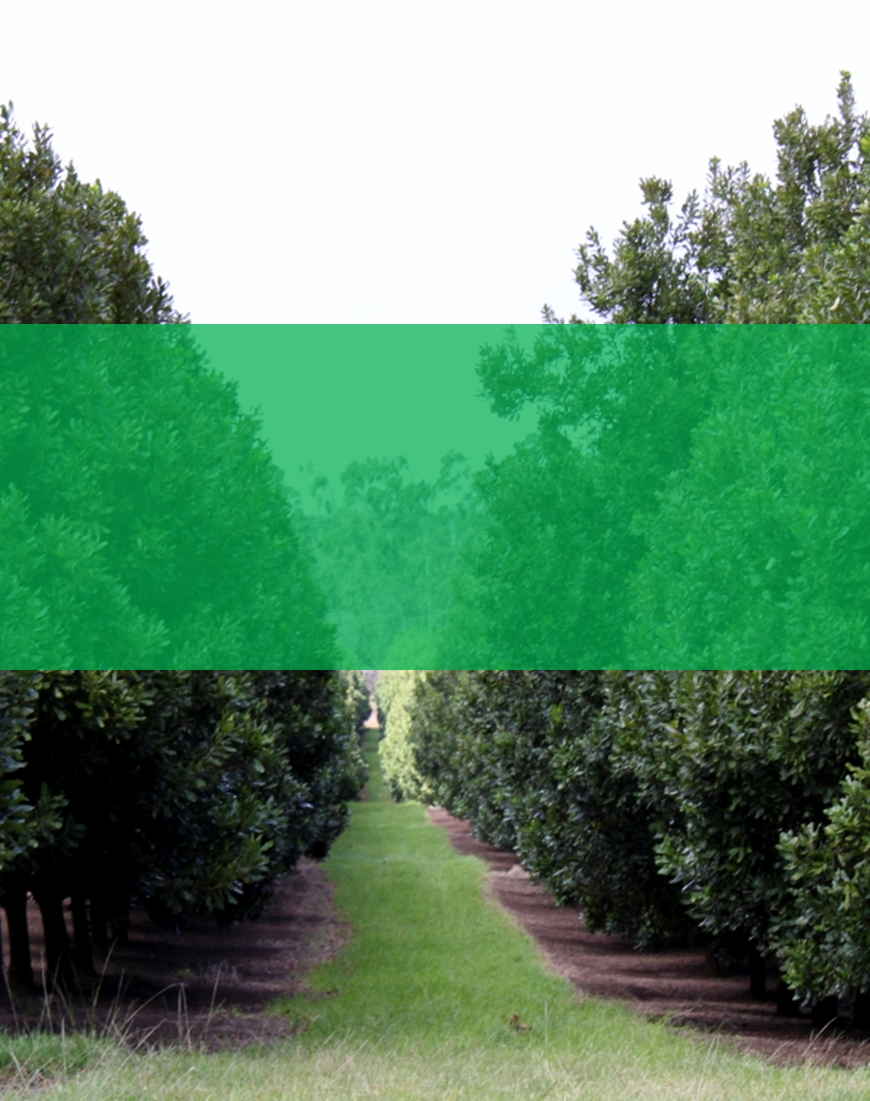
\includegraphics[scale=1]{frontcover}}} % Image background
\centering
\vspace*{5cm}
\par\normalfont\fontsize{35}{35}\sffamily\selectfont
\textbf{Harvest}\\
{\LARGE User Manual for Harvest System}\par % Book title
\vspace*{0.5cm}
{\Huge HTTP\_418}\par
\centering
\vspace*{0.5cm}
\begin{itemize}[label={}, noitemsep]	
		\Large
		\item \begin{center} Christiaan Saaiman, 12059138 \end{center}
		\item \begin{center} Michael Loosen, 14017254 \end{center}
		\item \begin{center} Elizabeth Bode, 14310156 \end{center}
		\item \begin{center} LC Meyers, 14024633 \end{center}	
\end{itemize}
\endgroup

%----------------------------------------------------------------------------------------
%	TABLE OF CONTENTS
%----------------------------------------------------------------------------------------

\chapterimage{orchard.png} % Table of contents heading image

\pagestyle{empty} % No headers

\tableofcontents % Print the table of contents itself

%\cleardoublepage % Forces the first chapter to start on an odd page so it's on the right

\pagestyle{fancy} % Print headers again

%----------------------------------------------------------------------------------------
%	CHAPTER 1
%----------------------------------------------------------------------------------------

\chapterimage{mangoes.png} % Chapter heading image

\chapter{Introduction}
	\section{About Harvest}
		We as HTTP\_418 created Harvest as an application to help farmers manage and control their crops, yields and workforce. Harvest is a two-part program that enables farmers to improve their farms productivity and management. The first part is a web interface with which the farmers create a profile and using this profile, the farmers will be able to create, view and edit farms, orchards, crops, foreman and workers. This web application will also provide the farmer with a means to view a heatmap of the farmer's crops, showing yield concentration as well as viewing indivdual worker and foreman performance. The second part of the application is a phone/tablet app, downloaded from the associated product's store, to be used by the foreman in the field as the crop gathering is in process. The foreman will update the data for each worker as they bring in crop yields and this information will be used in reports generated for the farmer to view his farm's statistics.
	\section{Installing Harvest}
		The only installing required will take place on the phone/tablet used by the foreman in the field.
		\begin{itemize}
			\item Navigate to your device's dedicated app store
				\subitem Google Play Store for Android
				\subitem App Store for iPhone or iPad
			\item Search for the Harvest app in the store
			\item Click on the install/get button and wait for the application to install on the device
		\end{itemize}
		Well done! You have completed the install process for the Harvest system.
	\section{Creating an Account on Harvest}
		\subsection{Creating an Account on the Website}
			Farmers can create an account simply by navigating to the website and then clicking on the large blue "Register Here" button found near the bottom of the page. The farmer then needs to enter his basic details and once he submits these details, his account will be created.
		\subsection{Creting an Account on the Mobile Application}
			*Not Implemented Yet - Will be similar to the website*
		In your computer's internet browser, navigate over to www.subtropharvest.co.za. It will look similar to this:
		\begin{figure}[H]
			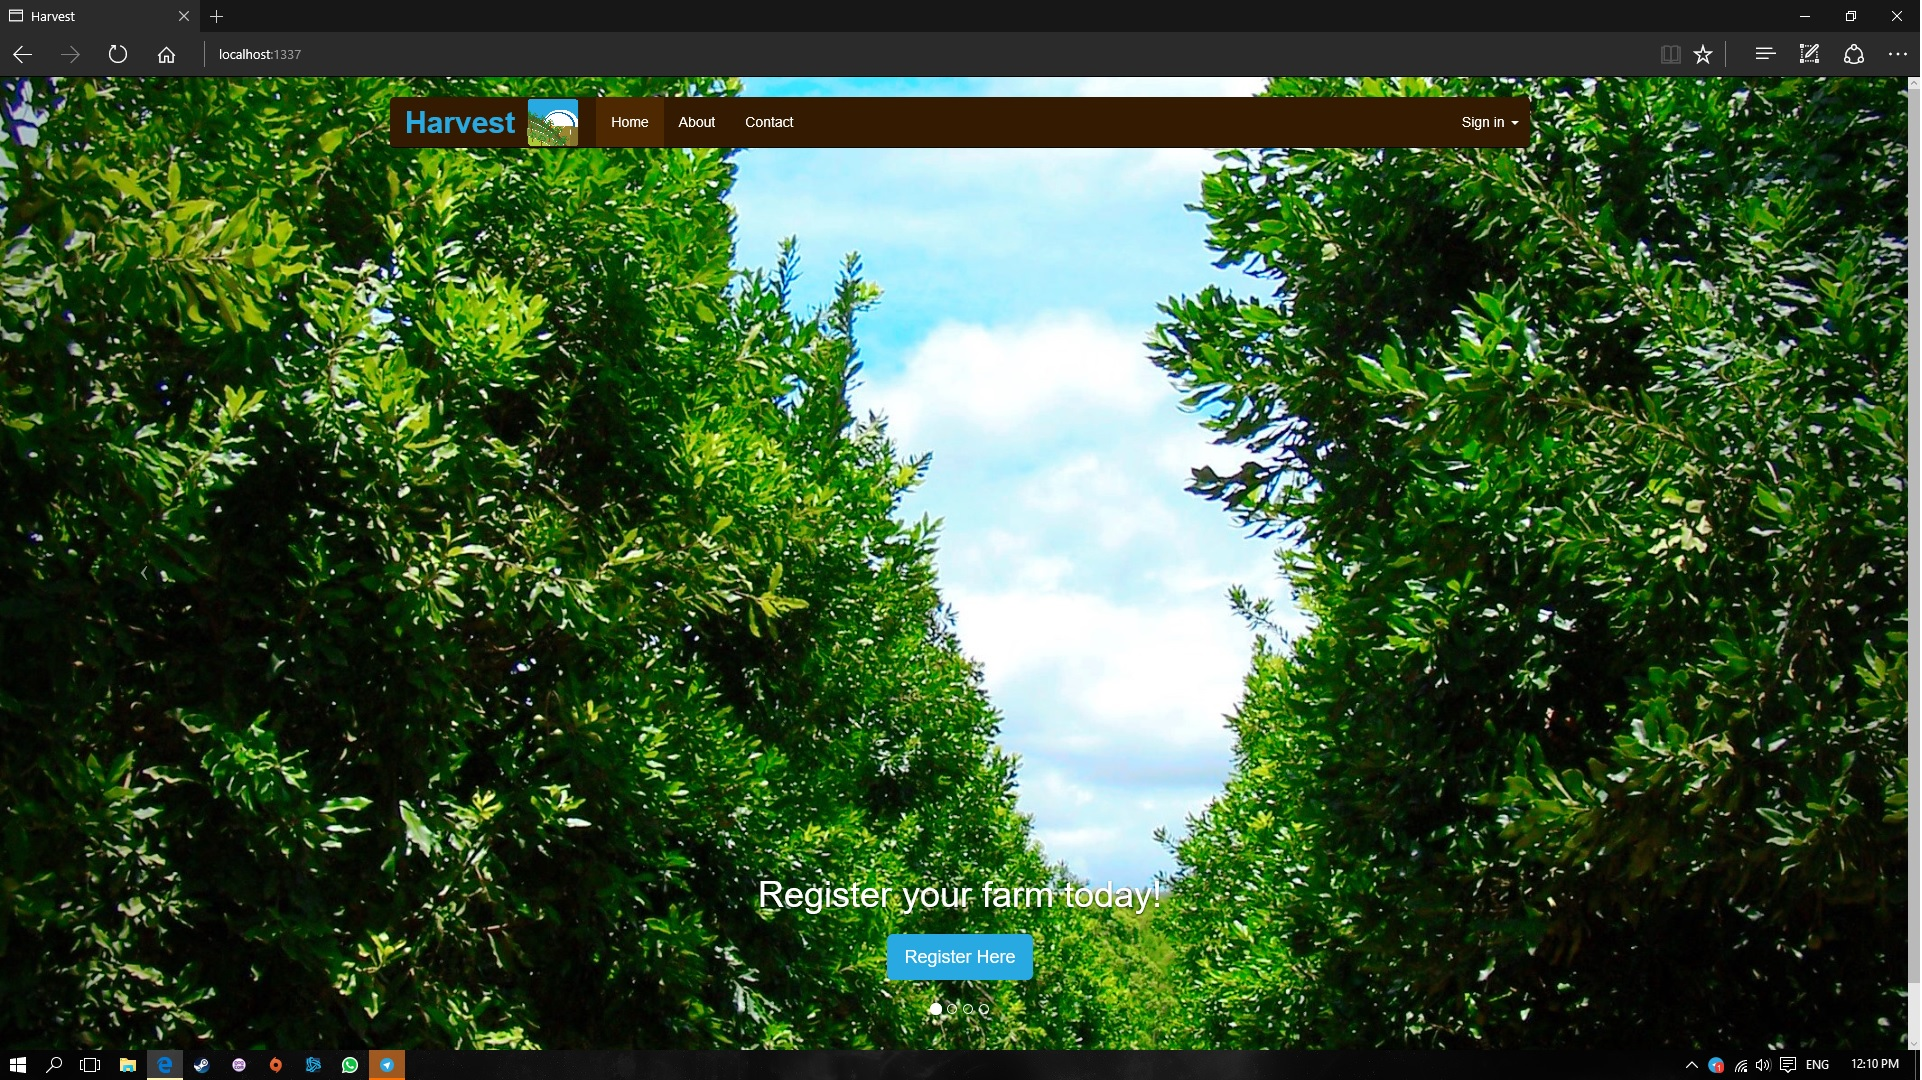
\includegraphics[scale=0.25]{Pictures/homescreen.jpg}\centering
			\caption{Homescreen of Harvest}
		\end{figure}
		On the screen, click the blue "Register" button, this will take you to this screen:
		\begin{figure}[H]
			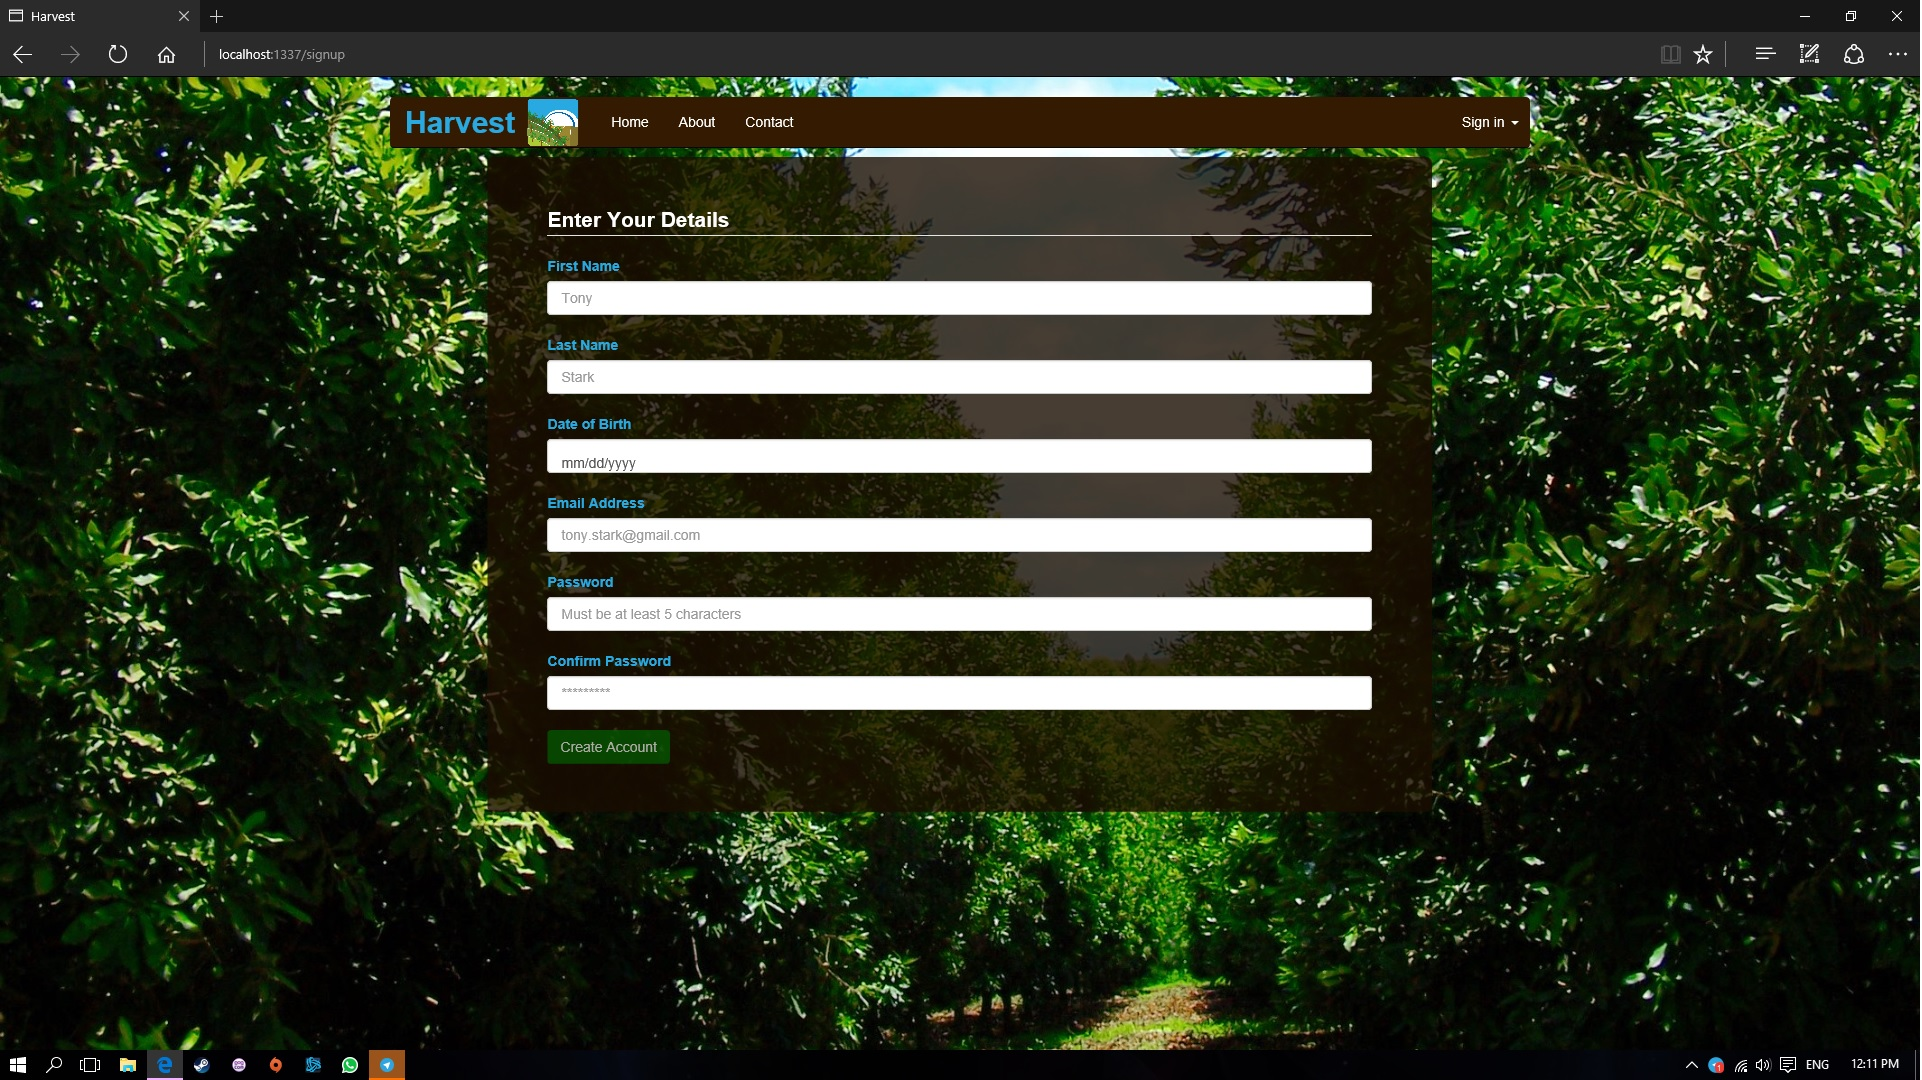
\includegraphics[scale=0.25]{Pictures/signup.jpg}\centering
			\caption{Sign up page}
		\end{figure}
		On the register page, please fill in all the fields with the correct data! Once you have completed that, click on the green "Create Account" button and, voilà! You are registered, can log in and start setting up the details to manage your farm!

%----------------------------------------------------------------------------------------
%	CHAPTER 2
%----------------------------------------------------------------------------------------
\chapterimage{macadamias.png}

\chapter{Using Harvest on your Farm}
	\section{What do you Need to Know as a Farmer?}
		% So you have an account John Deere, what now? *Insert app usage with foreman in the field explanation*
		
		Harvest enables you to monitor your farm in its entirety from your home. You simply need to register your farm on the website, log into the website using your credentials and then everything you need to know regarding your farm can be accessed. This includes monitoring your foremen's behaviour, monitoring the performance of your workers overall and at certain times during the day, mapping out the orchard blocks on your farm and monitoring the crop yields they bring in seasonally, annually or currently. The crop yield density can also be easily determined by viewing the heat map that can be generated for your farm. All the details of specific orchard blocks, such as the type of crop, the type of irrigation used, the frequency that cultivation takes place and the type of measurement used for determining yields, no longer needs to manually be recorded. Now everything can be viewed and modified in one place via a simple and user-friendly interface designed to suit your needs. The assignment of workers to specific foreman and allocating foremen to specific orchard blocks can also effortlessly be done using Harvest. All of this is simply done by assigning credentials to your foremen, which allows them to record and view their worker's performance. You can view all the worker performance data that your foremen have entered at any time assuming both you and your foreman are connected to the Internet. The use of unique credentials per foreman allows you to be able to monitor their whereabouts according to their GPS location. These credentials will be generated once you have added a new foreman to the system and then you are required to notify the foreman of these credentials.\newline\newline
		
		How does this benefit you in the long term? Harvest also allows for quick and easy generation of reports regarding worker performance, the amount of crop yield per orchard block, the revenue generated according to the yield collected in a specific season and the amount of time it takes to cultivate certain crops. This offers a multitude of benefits in regard to strategical planning for the future. Such planning includes, financial planning according to seasons, staff requirements and staff payment planning according to how much time is required for cultivating specific crops and planning where to plant certain crops according to higher yields collected in specific orchard blocks. The monitoring of worker performance can also highlight whether certain foremen aren't being strict enough with managing their workers or highlight the lack of crop yield collected either due to extreme weather conditions or them not working hard enough.\newline\newline
		
		As a farmer, you already have a lot of work on your hands monitoring large amounts of land and staff. Allow Harvest to make this process increasingly easier with the vast amount of benefits it offers.

		
	\section{Using Harverst on your Computer}
		\subsection{General Navigation - What do these buttons do?}
		\begin{itemize}
			\item \textbf{Logo Link} - This will navigate you back to the homepage of Harvest, which is the farm details page that contains all of the details related to your farm.
			\item \textbf{Your Farm dropdown} - This will drop down a list of options related to your farm.
			\begin{itemize}
				\item \textbf{View Farm Details Option} - This will navigate you to the farm details page.
				\item \textbf{Orchard Blocks Option} - This will navigate you to the orchard block details page.
				\item \textbf{Crop Types Option} - This will navigate you to the Crop Types details page.
				\item \textbf{Irrigation Types Option} - This will navigate you to the Irrigation Type details page.
				\item \textbf{Cultivation Frequencies Option} - This will navigate you to the Cultivation Frequency details page.
				\item \textbf{Yield Measurement Option} - This will navigate you to the Yield Measurement Type details page.
				\item \textbf{View Heat Map Option} - This will navigate you to the Heat Map page.
			\end{itemize}
			\item \textbf{Your Workers dropdown} - This will drop down a list of options related to the workers on your farm.
			\begin{itemize}
				\item \textbf{View Workers Option} - This will navigate you to the workers details page.
				\item \textbf{View Worker-Foreman Assignments Option} - This will navigate you to the worker-foreman assignments page.
			\end{itemize}
			\item \textbf{Your Foremen dropdown} - This will drop down a list of options related to the foremen on your farm.
			\begin{itemize}
				\item \textbf{View Foremen Option} - This will navigate you to the foremen details page.
				\item \textbf{View Foreman-Orchard Block Allocations Option} - This will navigate you to the foreman-orchard block allocations page.
				\item \textbf{Manage Foremen Shifts} - This will navigate you to the foremen shift details page.
			\end{itemize}
			\item \textbf{Your Reports dropdown} - This will drop down a list of options related to the Reports.
			\begin{itemize}
				\item \textbf{Worker Performance Option} - This will navigate you to a page that contains the report on a worker's performance.
				\item \textbf{Crop Yield Per Orchard Option} - This will navigate you to a page that contains the report on the crop yield related to an orchard.
				\item \textbf{Seasonal Yield Revenue Option} - This will navigate you to a page that contains the report on the seasonal yield revenue related to an orchard.
				\item \textbf{Time Taken to Cultivate Specific Crops Option} - This will navigate you to a page that contains the report on the time it took to cultivate specific crops.	
			\end{itemize}
			\item \textbf{Notification Bell} - This will navigate you to a page that contains all of your current notifications.
			\item \textbf{Edit Profile Link} - This will navigate you to a page that contains your profile details so that you can modify or update any incorrect details.
			\item \textbf{Log Out Link} - This will log you out of the system.
		\end{itemize}
	\section{Using Harvest to Manage your Staff}
		Harvest isn't just for your crops, yields and so, but for your people as well!! You can assign foreman to the mobile app that goes with the Harvest website. There the foreman can use the mobile app to monitor the worker performance of the workers that are assigned under them. The mobile app not only let's you monitor worker performance but also serves as a way to make sure your foreman do not leave the farm when they should not. The app features GPS tracking that can notify you through the website when a foreman leaves his post.
		
		*insert step by step guide and screenshots once implemented*


%----------------------------------------------------------------------------------------
%	CHAPTER 3
%----------------------------------------------------------------------------------------

\chapterimage{avocados.png}
\chapter{Troubleshooting}
	\section{When my App won't connect?}
		*Insert step by step instructions once server information is known"		
	\section{When my Profile won't display?}
		*Same as above*
	\section{When my Reports don't generate?}
		*Same as above*
%----------------------------------------------------------------------------------------
%	CHAPTER 4
%----------------------------------------------------------------------------------------

\chapterimage{litchis.png} % Chapter heading image

\chapter{Frequently Asked Questions[FAQ]}
	\section{App Related}
	*TODO, ask farmers questions at the expo in August to see what confused them.*
	\section{Computer Related}
	*TODO, ask farmers questions at the expo in August to see what confused them.*
	\section{Profile Related}
	*TODO, ask farmers questions at the expo in August to see what confused them.*
	
%----------------------------------------------------------------------------------------
%	CHAPTER 5
%----------------------------------------------------------------------------------------

\chapterimage{farmer.png} % Chapter heading image

\chapter{Still having Problems?}
	\section{Telephone}
		*Contact details for Subtrop*
	\section{Email}
		*Contact details for Subtrop*
	\section{Website}
		*Contact details for Subtrop*

%----------------------------------------------------------------------------------------
%	CHAPTER 6
%----------------------------------------------------------------------------------------

\chapterimage{mangoes2.png} %Chapter heading image

\chapter{Glossary of Terms}
	\section{Difficult Terms, Phrases and Other Lingo}
		\begin{itemize}
			\item \textbf{Cultivation Frequency} - The amount of time allocated for the crops to grow before harvesting again. Duration between harvests.
			\item \textbf{Irrigation Type} - The method that is used to water the crops.
			\item *Insert more difficult terms, phrases and lingo here as they are discovered.*
		\end{itemize}

\end{document}
